\section{Methodology}
\label{sec:method}

Perception is the part of \textsc{Sarbloh} that we developed most deliberately, so most of this section is about it: where it started (Section~\ref{sec:origins}), the eight designs we compared in a perception lab (Section~\ref{sec:lab}), what survived a held-out check (Section~\ref{sec:holdout}), and what the final engine computes (Section~\ref{sec:perception}). The last subsection (Section~\ref{sec:agent}) shows how the engine sits inside the whole agent (Figure~\ref{fig:overview}).

\subsection{Where Perception Started}
\label{sec:origins}

The first perception module, which we call the \emph{Legacy Encoder}, pushed a new observation into the context after every transition. It had four parts: the frame as a PNG in the ARC palette ($4\times$ nearest-neighbour, $256{\times}256$ pixels); a lettered board with one letter per colour, shown whole at the start of a level and afterwards only as the changed region with a 3-cell margin and numbered rows and columns; a segmentation list of 4-connected objects with id, colour, shape hash, bounding box, containment and adjacency, with HUD bars along the frame edge flagged; and one change line per transition (``\code{obj 4 moved dx=0 dy=-5; obj 9 vanished; 2 cells recoloured}''). It cost about 3{,}500 text tokens per frame.

Three early probes on the first level of \code{ls20} shaped it. They are qualitative, were logged from the author's own runs, and have no held-out score.
\begin{itemize}
    \item \textbf{Whole-frame picture versus cell deltas.} Sending only the changed cells is cheaper, but some actions change the game globally (stepping onto the modifier in \code{ls20} does), and a cell-delta view hides that. A whole-frame picture kept the global effect visible.
    \item \textbf{Picture plus segmentation text.} The model understood the frame precisely only when the segmentation list and the lettered board came beside the picture: the picture carries the global layout, the text carries exact positions.
    \item \textbf{Oracle briefing.} A frontier model played the same level twice, once from screenshots and the action space alone and once with a briefing we wrote by hand (action meanings, goal, mechanics, on-screen components). Without the briefing the game was wasted; with it the level was cleared in about six actions, against about ten for the author. Execution was adequate and understanding was the bottleneck (the ladder of Figure~\ref{fig:gemini}, Section~\ref{sec:motivation}).
\end{itemize}
The last probe set the target: an engine that writes the briefing itself, from the frame alone, for a game it has never seen.

\subsection{The Perception Lab: Eight Ways to Read One Frame}
\label{sec:lab}

We compared eight ways of presenting the same frame against the Legacy Encoder, one Python file each. All of them share one front end (screenshot, then an exact $64{\times}64$ palette grid, then the object list), so the only thing that changes is what is computed on top of the objects and how it is shown. The two test frames are the first levels of \code{ls20} (keyboard controls) and \code{r11l} (clicks). Understanding was graded against an answer key written and checked in the engine before any presentation ran: seven items per frame (spatial boundaries, mechanical linkages, agent identity, goal, gauges and so on) at two points each, 28 points in all, plus an intuition grade from 1 to 5. The kill rule was fixed in advance: drop a presentation that scores no better than the Legacy Encoder (3/28), or whose claims are wrong on about half or more of the held-out games.

\begin{figure*}[t]
\centering
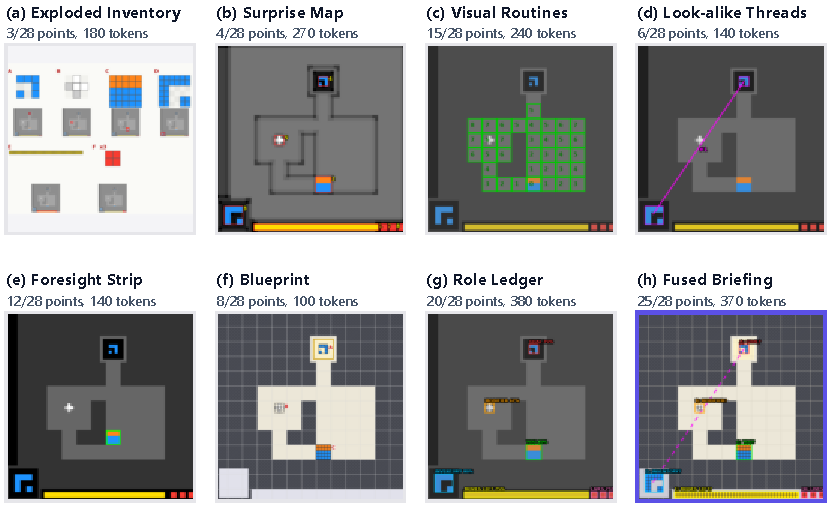
\includegraphics[width=\textwidth]{figures/perception_lab_gallery.pdf}
\caption{The image part of each candidate presentation for the opening frame of \code{ls20}, with its rubric score and its text cost per frame. (a) Exploded Inventory pulls out every object and stacks copies. (b) Surprise Map keeps colour only where the frame is unpredictable. (c) Visual Routines marks reachability, with the step count to each tile. (d) Look-alike Threads joins shapes that match under rotation, mirroring or scale. (e) Foresight Strip imagines the next frame (here, one step up). (f) Blueprint redraws floor, walls and lattice as a clean schematic. (g) Role Ledger tags each object with a guessed role and a confidence. (h) Fused Briefing, the presentation we kept, combines the blueprint with measured facts and tagged guesses.}
\label{fig:labgallery}
\end{figure*}

\begin{itemize}
    \item \textbf{Exploded Inventory} (3/28) pulls every object out of the frame, enlarges it, spaces the objects apart and stacks identical copies as $\times N$. The list is clean but attaches no meaning to anything.
    \item \textbf{Surprise Map} (4/28) ranks cells by how unpredictable their $3{\times}3$ neighbourhood is and flags broken symmetry. About 90\% of the frame is predictable texture, and the map caught the lopsided plus on \code{ls20}, but little else.
    \item \textbf{Visual Routines} (15/28), after Ullman, computes reachability by flood fill with step counts, what lies inside what, line tracing to attached objects, midpoints and alignment. On \code{r11l} it found the midpoint tether and the ring that fits a $5{\times}5$ object.
    \item \textbf{Look-alike Threads} (6/28) joins objects that are equal under rotation, flip, scale or recolouring and names the transform. On \code{ls20} it showed that the inventory icon is the goal shape turned $90^\circ$ and drawn at twice the size.
    \item \textbf{Foresight Strip} (12/28) imagines the next frame for each action from simple movement priors. On \code{ls20} it predicted all four moves and the gauge correctly, and on \code{r11l} its three-click plan solved the level.
    \item \textbf{Blueprint} (8/28) redraws the frame as a schematic: floor, walls, tile lattice, named shapes and the HUD moved to a side panel. It is the best map for navigation and says nothing about meaning.
    \item \textbf{Role Ledger} (20/28) guesses a role for every object (agent, goal, handle, gauge, lives) with a confidence and a one-action test. Every role was right on both frames.
    \item \textbf{Fused Briefing} (25/28) uses the Blueprint as its picture, states the Visual Routines and Look-alike Threads results as measured facts, and adds the Role Ledger guesses with their tests. Foresight Strip was dropped.
\end{itemize}

\begin{figure}[t]
\centering
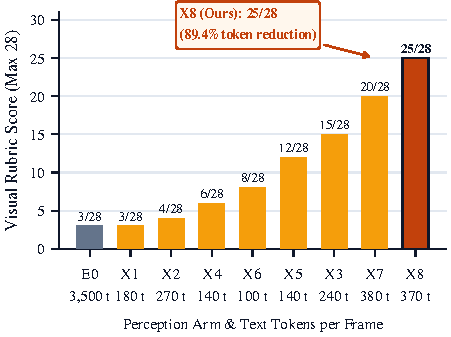
\includegraphics[width=\columnwidth]{figures/perception_lab.pdf}
\caption{Rubric score (of 28) and text tokens per frame for the Legacy Encoder and the eight presentations, on the two test frames. The Fused Briefing scores 25/28 against 3/28 for the Legacy Encoder at about a tenth of the text.}
\label{fig:lab}
\end{figure}

Exploded Inventory and Surprise Map did no better than the Legacy Encoder, at a tenth of its text, and were dropped as stand-alone presentations. What moved understanding most were the computed relations of Visual Routines and Look-alike Threads, which state facts a model cannot reliably read off a picture, and the Role Ledger, which gives the fastest gist. The Fused Briefing reached 25/28 at about 370 tokens per frame, 8.3$\times$ the Legacy Encoder's score with 89.4\% fewer text tokens. Two caveats apply. The grader was the same agent that built the presentations and knew both games, and no blind reader was used. The Fused Briefing was designed after the other eight were graded and was graded on the same two frames, so its score is optimistic.

\subsection{Held-Out Check: Facts Versus Guesses}
\label{sec:holdout}

We then checked the presentations on the 23 other official games, none of which had been used in the design. This check was graded by the engine rather than by hand (Table~\ref{tab:holdout}). Turning a screenshot into a grid generalised perfectly (23/23 games at 100\% cell accuracy). The guesses did not: they had effectively been fitted to the two test frames and were right about half the time or less on unseen games.

\begin{table}[t]
\centering
\small
\begin{tabular}{@{}L{0.55\columnwidth}L{0.36\columnwidth}@{}}
\toprule
Check on the 23 held-out games & Result \\
\midrule
Screenshot to grid, exact cells & 23/23 games \\
Agent identity, keyboard games & 6/14 games \\
Moves-left gauge found & 10/20 games \\
Click handles that respond & 7/29 handles \\
Keyboard foresight fully right & 1/16 games \\
\bottomrule
\end{tabular}
\caption{Held-out check of the single-frame guesses. For click handles, the guesses were good on \code{dc22} (2/2), \code{sb26} (4/4) and \code{ka59} (1/1) and bad on \code{lp85} (0/17). On two further keyboard games nothing moved on the first key press, so the agent-identity guess could not be checked.}
\label{tab:holdout}
\end{table}

This fixed the design rule of the engine: \emph{computed relations (reachability, enclosure, tethers and midpoints, alignment, shape equivalence) are stated as facts, because they are true by construction, whereas roles and dynamics from a single frame are stated as guesses, each with a one-action test that settles it}. One real action answers what a single-frame prior cannot. We did not run the Fused Briefing as a whole on the held-out games, and the lab reports no RHAE. The end-to-end effect of the engine on the agent is not isolated by an ablation: the trajectory of Section~\ref{sec:trajectory} changes several components at once.

\subsection{The Perception Engine}
\label{sec:perception}

The final engine is the Fused Briefing, rewritten to work directly on the grid inside the agent. It is about 1{,}500 lines of host-side NumPy and Pillow with no learned parameters. Over 225 real frames (the first frame and eight random actions on each of 25 offline games) it raised no errors, with a median of 42\,ms for the briefing and 40\,ms for the picture (maximum 0.38\,s for a briefing). For every environment transition it generates three synchronized representations sharing one persistent object identity space (Figure~\ref{fig:views}, Algorithm~\ref{alg:perceive}).

\begin{figure*}[t]
\centering
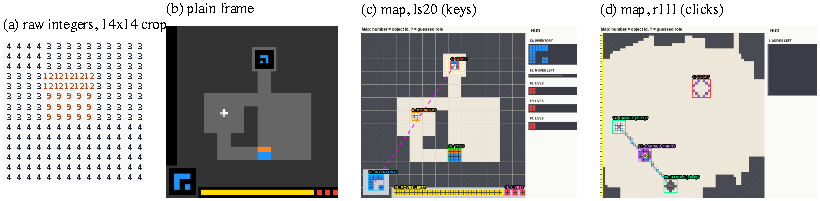
\includegraphics[width=\textwidth]{figures/perception_views.pdf}
\caption{Structural multimodal representation of an ARC-AGI-3 frame produced by the perception engine. (a) Conventional serialization provided to language models: an unparsed matrix of discrete integer tokens ($14{\times}14$ crop of a $64{\times}64$ frame). (b) Rendered 2D visual frame. (c, d) Affordance-annotated perception maps generated for the opening frames of \code{ls20} (discrete keyboard controls) and \code{r11l} (continuous spatial clicks). Traversal floor surfaces are rendered in light tones, impenetrable barriers are hatched, and peripheral HUD panels are isolated and scaled on the right. Tracked entities display persistent integer IDs alongside scored affordance roles. Magenta dashed threads indicate dihedral shape equivalence under rotation and scaling; yellow rings indicate mechanical midpoint tethers.}
\label{fig:views}
\end{figure*}

\paragraph{View 1: Morphological Segmentation, Tracking, and Change Ledgers.}
The background canvas is identified via the modal color index across the frame. All remaining 4-connected monochromatic components are segmented into discrete entities characterized by spatial bounding boxes, exact pixel masks, adjacency matrices, and topological containment hierarchies. On the initial frame of a level, entities are assigned persistent identifiers in standard raster reading order. On subsequent frames, an invariant bipartite matching algorithm tracks entity persistence across five sequential priority passes:
\begin{enumerate}
    \item \emph{Rigid Invariance}: Identical shape hash, color index, and spatial coordinates.
    \item \emph{Spatial Translation}: Identical shape hash and color index with translated coordinates.
    \item \emph{State Recoloring}: Identical shape hash and spatial coordinates with altered color index.
    \item \emph{Morphological Deformation}: Identical color index with significant spatial overlap ($>50\%$ IoU).
    \item \emph{Novel Component Instantiation}: Entities unmapped by preceding passes are instantiated with fresh unique IDs.
\end{enumerate}
Consequently, symbolic references such as \code{objects[10]} within the agent's Python kernel refer to the identical physical entity across the entire level lifetime. The spatial grid is transcribed into a lettered alphanumeric matrix with explicit row and column headers. Sequential actions append a differential change ledger formatted as: ``\code{\#12 A4(right): 6 cells altered at r10-12 c20-25; HUD altered (1 cell)}''. Environmental changes within the peripheral 3-cell screen boundary are partitioned into HUD telemetry, preventing minor status updates (e.g., action counter decrements) from obfuscating playfield invariants.

\paragraph{View 2: Layout Decomposition and Verified Geometric Invariants.}
The structural briefing decomposes the playfield into macroscopic functional layouts. Color partitions spanning $>8\%$ of total frame area are classified as terrain. The remaining visual structure is decomposed into functional primitives: linear corridors, peripheral boundary gauges, composite multi-colored assemblies (clustered via union-find over 8-connected components), panel icons, and dotted figures.

Conditioned on this layout, the engine computes seven categories of mathematically verifiable \textsc{Measured Invariants}, true by geometric construction:
\begin{itemize}
    \item \textbf{Lattice Reachability}: Breadth-first search (BFS) over detected spatial lattices computes exact traversal distances from potential agent entities to all interactive targets (e.g., ``\code{obj 6 reachable in 6 steps}''; ``\code{enclosure entry accessible at bottom face in 5 steps}'').
    \item \textbf{Topological Enclosure}: Detection of closed boundaries enclosing empty spatial cavities, mapped against entities matching those cavity dimensions.
    \item \textbf{Midpoint Tethers}: Identification of linear linkages spanning entity pairs, calculating mechanical centerpoints (e.g., ``\code{obj 25 held at midpoint of obj 16 and 36; endpoint translation forces midpoint translation}'').
    \item \textbf{Coordinate Collinearity}: Verification of shared row or column alignments between key landmarks.
    \item \textbf{Dihedral Affine Symmetries}: Identification of shape equivalence under the dihedral group $D_4 \times \mathbb{Z}^+$ (spanning reflection, 90$^\circ$ rotations, and integer scaling), identifying cross-scale functional analogues (e.g., ``\code{obj 12 is a 2$\times$ scaled reflection of goal obj 4}'').
    \item \textbf{Multiplicity Counters}: Clusters of identical morphological instances, parsed as discrete countable sets (e.g., life indicators, consumable resources).
    \item \textbf{Color Polarity Asymmetries}: Detection of morphologically symmetric entities exhibiting asymmetric chromatic distributions, marking directional orientation or active operational state.
\end{itemize}

\paragraph{Affordance Role Induction and Minimal Falsification Probes.}
Subsequent to invariant verification, non-terrain components are evaluated against eight canonical game-design affordance roles via weighted evidence scoring (Table~\ref{tab:roles}). To eliminate the risk of hallucinated mental models, the engine couples each inferred role hypothesis with an explicit, single-action falsification probe:
\begin{table}[t]
\centering
\footnotesize
\setlength{\tabcolsep}{3.5pt}
\begin{tabular}{@{}L{0.22\columnwidth}L{0.37\columnwidth}L{0.35\columnwidth}@{}}
\toprule
Affordance Role & Evidentiary Priors (Scored) & Unit Falsification Probe \\
\midrule
\textsc{Player / Agent} & Compact, multi-chromatic, unique, lattice-aligned & Issue 1 directional action: verify 1-tile translation \\
\textsc{Target Goal} & Hollow receptor, bounding enclosure, HUD shape matching & Transport matching entity into enclosure \\
\textsc{Action Gauge} & Elongated peripheral bar spanning screen margin & Issue arbitrary action: verify 1-unit reduction \\
\textsc{Life Counter} & Multiple identical glyphs in peripheral HUD & Observe count upon episode reset or hazard \\
\textsc{Inventory} & Isolated HUD glyph mirroring playfield entity & Observe glyph after interacting with modifier \\
\textsc{Modifier} & Compact symbol exhibiting chromatic asymmetry & Traverse onto entity: verify inventory mutation \\
\textsc{Actuator Handle} & Tether endpoint; chromatic toggle pair & Issue coordinate click: verify spatial jump \\
\textsc{Coupled Cargo} & Mechanically constrained between two tether handles & Translate handle: verify proportional shift \\
\bottomrule
\end{tabular}
\caption{Affordance role induction rules. Each hypothesis is presented with evidentiary confidence and an explicit single-action falsification test, ensuring erroneous hypotheses are refuted at minimal action cost.}
\label{tab:roles}
\end{table}

The natural language briefing is bounded to 30 lines by default, allocating at most one-third of that budget to role hypotheses and sharing the rest among the invariant categories so that no single kind of fact can fill it; facts touching the guessed agent and goal come first, and the remainder are counted (``\code{+N more facts}'') and stay available through \code{observe().briefing}. Complete structured briefings are provided in Appendix~\ref{app:briefings}.

\paragraph{View 3: Structured Affordance Map.}
The spatial map (Figure~\ref{fig:views}c,d) renders abstracted semantic structure rather than raw pixels: accessible terrain is rendered in pale tones, impassable walls are hatched, detected lattice grids are overlaid as fine lines, and all entities are bordered by role-colored bounding markers labeled ``\code{id: ROLE?}''. Look-alike symmetries under $D_4 \times \mathbb{Z}^+$ are joined via dashed chromatic threads, while mechanical tether linkages display midpoint concentric rings. Peripheral HUD panels are isolated and magnified on the right. Crucially, natural language annotations are excluded from image pixels and transmitted strictly as structured text, maximizing token efficiency and eliminating visual OCR errors.

\paragraph{Observation Scheduling.}
The full multimodal observation (briefing text, alphanumeric grid, and rendered map) is transmitted at level inception, following context window purges, and when the agent calls \code{observe()} after acting, at most once per state. Following intermediate actions, the agent receives an abbreviated observation: the differential change ledger, a cropped alphanumeric window centered on the modified coordinate region with a 3-cell margin, and the updated visual map, consuming fewer than 600 tokens. The complete object table is retained host-side and queried on-demand via Python kernel calls (\code{observe().objects}).

\paragraph{Hardening inside the agent.}
Two problems appeared only once the engine ran on live play. First, the test for a tile lattice flipped during play: \code{ls20} lost its $5{\times}5$ grid after one move, because the gauge in the status box added off-grid edges, and \code{ka59} lost its $3{\times}3$ grid whenever the agent touched another object. Status boxes are now left out of the test and the level's previous lattice is kept while it still fits, which removed all flips on the 225 frames. Second, ``X is directly above Y'' facts crowded out everything else: on \code{tr87} they filled 27 of the 30 briefing lines (68 facts in all, and 792 on \code{bp35}). A fixed cap also deleted facts from \code{observe().briefing}, so we kept every alignment fact, put those touching the guessed agent and goal first, and let each kind of fact take only its share of the lines shown.

\begin{algorithm}[t]
\caption{\textsc{Perceive}: Deterministic Frame-to-Modality Mapping}
\label{alg:perceive}
\KwIn{Raw grid $g_t \in \{0..15\}^{H\times W}$, persistent tracker $T$, lattice prior $\Lambda'$, legal actions $\mathcal{A}$}
\KwOut{Structured briefing $B$, tracked entities $O$, visual map $M$, differential change $\delta$}
$O \gets \textsc{MorphologicalSegmentation}(g_t)$\;
$(O, \delta) \gets T.\textsc{BipartiteMatch}(O)$ \Comment*[r]{temporal identity persistence}
$\mathcal{T} \gets \{c \in \{0..15\} : |g_t{=}c| > 0.08\,HW\}$ \Comment*[r]{terrain segmentation}
$L \gets \textsc{ExtractLayout}(g_t, \mathcal{T})$\;
\ForEach{entity $e \in L$}{
  $e.\mathit{is\_hud} \gets \textsc{IsPeripheralBoundary}(e)$\;
  $e.\mathit{id} \gets \textsc{MajorityOverlapId}(e, O)$\;
}
$e_{\text{agent}} \gets \textsc{IdentifyCandidateAgent}(L, \mathcal{A})$\;
$\Lambda \gets \textsc{DetectLattice}(L) \textbf{ or } \Lambda'$\;
$F \gets \textsc{BFSReach}(e_{\text{agent}}, \Lambda) \cup \textsc{Enclosures}(L)$\;
$F \gets F \cup \textsc{Tethers}(L) \cup \textsc{Symmetries}_{D_4\times\mathbb{Z}^+}(L)$\;
\ForEach{entity $e \in L$}{
  $\boldsymbol{\sigma}_e \gets \textsc{ScoreAffordances}(e, F, \mathcal{A})$\;
  $\hat{\rho}_e \gets \arg\max_r \boldsymbol{\sigma}_e[r], \quad p_e \gets \boldsymbol{\sigma}_e[\hat{\rho}_e] / (1 + \sum_r \boldsymbol{\sigma}_e[r])$\;
}
$B \gets \textsc{FormatInvariants}(F)$\;
$B \gets B \,\|\, \textsc{FormatHypotheses}(\hat{\boldsymbol{\rho}}, \boldsymbol{p}, \textsc{Tests}(\hat{\boldsymbol{\rho}}))$\;
$M \gets \textsc{RenderAffordanceMap}(L, \hat{\boldsymbol{\rho}}, F)$\;
\Return{$(B, O, \textsc{ToAlphanumeric}(g_t)), M, \delta$}
\end{algorithm}

\subsection{The Overall \textsc{Sarbloh} Agent}
\label{sec:agent}

\begin{figure*}[t]
\centering
\resizebox{\textwidth}{!}{%
\begin{tikzpicture}[
  font=\sffamily\footnotesize, >={Stealth[length=2.2mm]},
  box/.style={draw=ink!80, rounded corners=3pt, fill=white, minimum height=7.5mm, inner sep=3.5pt, align=center, line width=0.55pt},
  hot/.style={box, fill=soft, draw=ours, line width=0.85pt},
  cool/.style={box, fill=softb, draw=base, line width=0.75pt},
  lab/.style={font=\sffamily\scriptsize, text=ink!90, align=center},
  flow/.style={->, draw=ink!75, line width=0.65pt},
  hotflow/.style={->, draw=ours, line width=0.95pt},
]
% --- one game session -------------------------------------------------------------------------------------------
\node[cool, minimum width=21mm] (game) at (0,0) {\textbf{ArcHost}\\[-1pt]{\scriptsize Environment sandbox,}\\[-1pt]{\scriptsize lossless step ledger}};
\node[hot, minimum width=27mm, right=9mm of game] (seg) {\textbf{1. Segment + Track}\\[-1pt]{\scriptsize 4-connected components,}\\[-1pt]{\scriptsize bipartite identity tracking}};
\node[hot, minimum width=27mm, right=3mm of seg] (layout) {\textbf{2. Layout Parsing}\\[-1pt]{\scriptsize terrain, panels, HUD,}\\[-1pt]{\scriptsize composite entities}};
\node[hot, minimum width=27mm, right=3mm of layout] (measure) {\textbf{3. Invariant Engine}\\[-1pt]{\scriptsize reachability, containment,}\\[-1pt]{\scriptsize tethers, $D_4 \times \mathbb{Z}^+$ symmetry}};
\node[hot, minimum width=27mm, right=3mm of measure] (guess) {\textbf{4. Affordance Scorer}\\[-1pt]{\scriptsize operational hypotheses,}\\[-1pt]{\scriptsize minimal unit falsification}};
\node[hot, minimum width=24mm, right=3mm of guess] (render) {\textbf{5. Multimodal View}\\[-1pt]{\scriptsize spatial map, coordinate grid,}\\[-1pt]{\scriptsize differential change line}};
\begin{scope}[on background layer]
\node[draw=ours, dashed, rounded corners=5pt, fill=ours!5, fit=(seg)(render), inner sep=6pt, label={[lab, text=ours, yshift=-1pt]above:\textbf{Deterministic Perception Engine} (Host-side, zero parameters, $\mathcal{O}(HW)$, tens of ms per frame on 1 CPU core)}] (pe) {};
\end{scope}

\node[box, minimum width=35mm, below=14mm of render.south east, anchor=north east] (ctx) {\textbf{Append-Only Context}\\[-1pt]{\scriptsize monotonic growth invariant,}\\[-1pt]{\scriptsize 98.4\% KV prefix-cache hit rate}};
\node[cool, minimum width=35mm, left=8mm of ctx] (llm) {\textbf{Qwen3.8-Flash-Next}\\[-1pt]{\scriptsize 125B MoE (6B active per token)}\\[-1pt]{\scriptsize AutoRound W4A16, SGLang + EAGLE}};
\node[box, minimum width=45mm, left=8mm of llm] (kernel) {\textbf{IPython Execution Kernel}\\[-1pt]{\scriptsize \code{observe()} \quad \code{await play(path, predict)}}\\[-1pt]{\scriptsize Persistent symbolic memory dictionaries}};

\draw[flow] (game) -- node[lab, above]{$g_t$} (seg);
\draw[flow] (seg) -- (layout);
\draw[flow] (layout) -- (measure);
\draw[flow] (measure) -- (guess);
\draw[flow] (guess) -- (render);
\draw[hotflow] (render.south) -- node[lab, right]{aligned views} (render.south |- ctx.north);
\draw[flow] (ctx) -- node[lab, above]{prefix prompt} (llm);
\draw[flow] (llm) -- node[lab, above]{Python code} (kernel);
\draw[hotflow] (kernel.west) -| node[lab, pos=0.75, left, align=right]{speculative path execution\\(auto-preemption on discrepancy)} (game.south);

% --- run level -------------------------------------------------------------------------------------------------
\node[box, minimum width=35mm, below=10mm of llm] (sched) {\textbf{Utility Priority Scheduler}\\[-1pt]{\scriptsize 25 concurrent games, 10 GPU slots,}\\[-1pt]{\scriptsize marginal RHAE utility $\times$ hope decay}};
\node[box, minimum width=35mm, right=8mm of sched] (cur) {\textbf{Cross-Level Curator}\\[-1pt]{\scriptsize relational lessons graph,}\\[-1pt]{\scriptsize falsified hypothesis blacklist}};
\node[box, minimum width=45mm, left=8mm of sched] (srv) {\textbf{Self-Healing Runtime Watchdog}\\[-1pt]{\scriptsize zero-progress stall detection,}\\[-1pt]{\scriptsize wall-clock budgeted recovery chain}};
\draw[flow, dashed] (sched) -- (llm);
\draw[flow, dashed] (cur.north) -- ++(0,4.5mm) -| (kernel.south east);
\draw[flow, dashed] (srv) -- (sched);
\end{tikzpicture}}
\caption{System architecture of \textsc{Sarbloh}. The host runtime encapsulates the environment sandbox. Each observation frame is processed by the deterministic perception engine (orange), generating three aligned modalities ingested into a strictly monotonic, append-only context window. The agent reasons exclusively by executing code within an embedded IPython kernel, inspecting state via \code{observe()} and committing speculative trajectories via \code{await play()}. Across 25 concurrent game sessions, a single enterprise GPU is dynamically multiplexed via an optimal utility-based priority scheduler.}
\label{fig:overview}
\end{figure*}

Figure~\ref{fig:overview} puts the perception engine in the context of the whole agent. The runtime orchestrates 25 concurrent game sessions multiplexed across a single GPU. For each environment, the host sandbox intercepts the raw frame and the perception engine turns it into the aligned views described above. An append-only context manager streams these views into the model prompt while preserving prefix-cache residency. The reasoning backbone works through an embedded IPython kernel, modelling the environment in Python and executing multi-step paths by speculative execution. The remaining components are described below.

\paragraph{Speculative code-as-action.}
\textsc{Sarbloh} acts exclusively through a single persistent IPython execution kernel, extending the CodeAct paradigm \citep{wang2024codeact}. Within the execution REPL, \code{observe()} returns the current multimodal observation state as Python data structures. Action commitment is performed exclusively through a speculative execution primitive:
\begin{center}
{\small\code{await play(path, predict=transition\_model)}}
\end{center}
where \code{path} denotes a planned sequence of up to 100 candidate actions, and \code{predict} specifies an optional programmatic world model $\hat{f}(s, a) \to \hat{s}$. In preliminary iterations, providing the model with separate, distinct tools for code execution and action submission induced severe mode-switching loops, where the agent vacillated between code generation and single-step action queries. Unifying action commitment directly into the Python kernel enabled the model to synthesize algorithmic state machines, execute trajectory searches (BFS/DFS), and commit complete planned trajectories within a single execution turn.

\begin{algorithm}[t]
\caption{\textsc{Play}: Speculative Path Execution with Runtime Preemption}
\label{alg:play}
\KwIn{Action trajectory $m_1, \dots, m_K$, optional transition model $\hat{f}$}
$s \gets \textsc{Observe}()$; \quad $\textit{discrepancy} \gets \varnothing$\;
\For{$i \gets 1$ \KwTo $K$}{
  \lIf{$\hat{f} \neq \varnothing$}{$\hat{s} \gets \hat{f}(s.\text{board}, m_i)$}
  $r \gets \textsc{ArcHost}.\textsc{CommitAction}(m_i)$ \Comment*[r]{verified execution}
  $s' \gets \textsc{Observe}()$\;
  \If{$\hat{f} \neq \varnothing$ \textbf{and} $\textit{discrepancy} = \varnothing$ \textbf{and} $\textsc{Diff}_{\neg\text{HUD}}(\hat{s}, s'.\text{board}) \neq \varnothing$}{
    $\textit{discrepancy} \gets (i, m_i, \text{mismatched\_cells})$\;
    $\textsc{ArcHost}.\textsc{SetShortThinkingBudget}()$\;
  }
  \If{level\_completed \textbf{or} game\_over \textbf{or} $s'$ visited in current attempt \textbf{or} barrier hit twice}{
    \textbf{break}\;
  }
  $s \gets s'$\;
}
\Return{change\_ledgers, \textit{discrepancy}, $s'$}
\end{algorithm}

Algorithm~\ref{alg:play} defines the speculative execution contract. Prediction discrepancies between the agent's internal model $\hat{s}$ and the true environment state $s'$ do not terminate execution prematurely; rather, discrepancies are registered with exact coordinate diffs, triggering a shortened thinking budget on the subsequent turn to facilitate rapid local hypothesis refinement. 

Conversely, speculative execution is immediately preempted whenever runtime telemetry confirms that further action commitment is deleterious. The \emph{state revisit leash} monitors the hash of playfield configurations (excluding the peripheral 3-cell HUD border): if the agent reproduces a state visited earlier within the current attempt, the execution loop is immediately aborted, arresting cyclical wandering. Furthermore, voluntary episode resets are bounded to three per level, eliminating pathological restart loops observed in unconstrained baselines. When evaluated post-hoc across offline trajectories, the revisit leash successfully suppressed 2,331 redundant exploratory actions across 9,913 total steps without truncating a single successful solution path.

\paragraph{Monotonic append-only context.}
Our deployed backbone architecture integrates Gated DeltaNet linear recurrent layers with sparse multi-head attention \citep{yang2024gated}. While linear attention provides exceptional generation speed, its recurrent state representation imposes a rigid operational invariant: the model serving engine can only resume generation from state checkpoints recorded at the terminal boundary of prior requests. Any retrospective modification to historical tokens---such as replacing stale visual images or updating historical messages---invalidates the recurrent state, triggering expensive full prefill recomputation.

In early deployments, unconstrained prompt rewriting resulted in catastrophic cache degradation: 3,283 of 5,599 sequential requests experienced 0\% prefix cache reuse, requiring continuous prefill that saturated GPU bandwidth. We resolved this systems bottleneck by enforcing a strictly \emph{monotonic, append-only context protocol}. Generation histories retain all preceding reasoning traces, newly rendered images are appended as discrete immutable messages following the action output that produced them, and state modifications are appended strictly as delta logs. As demonstrated in Table~\ref{tab:telemetry}, this append-only invariant raised prompt prefix-cache utilization to \textbf{98.4\%} across full nine-hour runs, effectively rendering the serving system decode-bound.

\paragraph{Deterministic context drainage.}
When cumulative context length surpasses 118k tokens, the runtime executes a deterministic context drainage routine, discarding the oldest conversational turns in code until total length falls below 55k tokens. Unlike prior agent frameworks that rely on recursive model-generated summaries \citep{knutsen2026arcgentica}, our purge routine uses zero LLM calls, completely avoiding the accumulation of hallucinated summaries. The initial system prompt is permanently pinned, and the active symbolic memory state and Python code graph are re-injected as a clean prefix checkpoint (Algorithm~\ref{alg:loop}, Line~3).

\paragraph{Working memory and relational graph.}
The agent maintains working memory within four structured dictionaries persisted inside the IPython kernel: \code{GOAL}, \code{PLAN}, \code{HYPOTHESES}, and \code{FINDINGS}. These structures are retained across level transitions, ensuring that inductive knowledge acquired in early levels remains accessible when solving complex compositional stages. A fifth structure, \code{SKILLS}, is populated via a post-level \emph{curator}. Following each completed level, a fast structured JSON call evaluates verified versus refuted hypotheses, updating a cross-level relational lessons graph and maintaining an explicit blacklist of falsified rules to prevent the re-generation of refuted behavioral hypotheses. Live abstract syntax tree (AST) analysis inspects kernel variables following each cell execution, appending a single telemetry line summarizing defined or broken functional dependencies.

\begin{algorithm}[t]
\caption{\textsc{Session}: Turn Execution Loop for an Individual Game}
\label{alg:loop}
\While{execution budget active \textbf{and not} terminal\_state}{
  \For{$j \gets 1$ \KwTo 12}{
    \lIf{$|\text{context}| > 118\text{k}$}{drain oldest turns to 55k; re-insert pinned memory}
    $y \gets \textsc{LLM}(\text{context})$ \Comment*[r]{98.4\% prefix-cached}
    execute IPython code cells in $y$; append execution output, new visual map, state diffs\;
    \lIf{action committed to host \textbf{or} thinking tokens $> 16\text{k}$}{\textbf{break}}
  }
  $\textsc{Scheduler}.\textsc{YieldSlot}()$ \Comment*[r]{yield GPU slot after quantum}
  \lIf{level\_completed}{\textsc{CurateKnowledge}(); update skill graph}
}
\end{algorithm}

\paragraph{Model quantization and serving runtime.}
\textsc{Sarbloh} deploys Qwen3.8-Flash-Next, an advanced 125B parameter Mixture-of-Experts (MoE) architecture activating 6B parameters per token, featuring hybrid Gated DeltaNet and sparse attention layers. The model is quantized to W4A16 precision using AutoRound \citep{cheng2023autoround} and served via SGLang \citep{zheng2024sglang} with EAGLE speculative decoding \citep{li2024eagle} (configured with 3 draft speculative tokens), FP8 KV caching, and a 136k context window. Each game turn is allocated a 12k token generation ceiling. A self-healing watchdog monitors serving process health: servers that experience thread hangs (detected when token generation counters cease incrementing despite active client requests) are immediately terminated via stack dumps and restarted along a staged profile fallback chain, with restart budgets metered strictly by remaining wall-clock execution time.

\paragraph{Utility-driven priority scheduler.}
All 25 games are instantiated concurrently at runtime start, but active GPU access is restricted to 10 concurrent serving slots to prevent KV-cache thrashing. Slot allocation is governed by a dynamic utility-driven priority function. For a game session currently evaluating level $L+1$ of $n$, having expended $t$ generation tokens and $a$ actions on the active level, its priority index $\pi$ is computed as:
\begin{equation}
\pi = \left(\frac{L+1}{\frac{n(n+1)}{2}} \cdot \left(\frac{h}{h+a}\right)^2 + \gamma_{\text{tail}}\right) \cdot 2^{-\left(\left(\frac{t}{\tau}\right)^2 + \left(\frac{a}{\alpha}\right)^2\right)},
\label{eq:priority}
\end{equation}
where $h=25$ represents the median human baseline constant, $\tau=40\text{k}$ tokens denotes the token exhaustion threshold, $\alpha=115$ actions denotes the exploration action limit, and $\gamma_{\text{tail}}=0.05$ ensures non-zero starvation prevention. The first factor formalizes the expected marginal RHAE reward attainable upon clearing the active level, discounted quadratically by accumulated action expenditure. The second factor models an exponential \emph{progress hope function}: games that consume substantial compute or action budgets without achieving state transitions experience rapid priority decay, gracefully yielding GPU resources to productive game sessions. Upon clearing a level, a game's counters are reset and its priority is immediately re-evaluated.
